\documentclass[12pt,a4paper]{report}
\usepackage[utf8]{inputenc}
\usepackage{graphicx}
\usepackage{amsmath}
\usepackage{amssymb}
\usepackage{hyperref}
\usepackage{listings}
\usepackage{caption}
\usepackage{subcaption}
\usepackage{tocloft}
\usepackage{titlesec}
\usepackage[numbers,super]{natbib}
\usepackage{booktabs}
\usepackage{xcolor}
\usepackage{listings-rust}
\usepackage{listings-json}
\usepackage[romanian]{babel}
\usepackage[brazilian]{cleveref}
\usepackage{float}
\usepackage{verbatim}

\lstset{language=Rust, style=colouredRust}

\titleformat{\chapter}[hang]
  {\normalfont\huge\bfseries}{\thechapter.}{1em}{}

\setlength{\cftbeforetoctitleskip}{-50pt}
\titlespacing*{\chapter}{0pt}{-50pt}{10pt}

\begin{document}

\begin{titlepage}
      \centering
      \vspace*{1cm}

      \Huge
      \textbf{Sistem de Clasificare Malware Android}

      \vspace{0.5cm}
      \LARGE
      Lucrare de Licență

      \vspace{1.5cm}

      \textbf{Crețu Vlad-Sebastian}

      \vfill

      \Large
      Coordonator: Dr. Ing. Aciu Răzvan-Mihai

      \vspace{0.8cm}

      
\includegraphics[width=0.4\textwidth]{visuals/university_logo.jpg}

      Universitatea Politehnica Timișoara\\
      Facultatea de Automatică și Calculatoare\\
      2024

\end{titlepage}

\tableofcontents


\chapter{Introducere}
Lucrarea se concentrează pe dezvoltarea unui sistem de clasificare multi-label a fișierelor APK\cite{apk-file-format-wiki} folosind 5 componente principale:
\begin{itemize}
      \item Bibliotecă de preprocesare a datelor realizată folosind limbajul de programare Rust\cite{rustlang},
            care se ocupă de extragerea permisiunilor și secvențelor de cod din fișierele APK.
      \item Model machine-learning de clasificare realizat folosind biblioteca Tensorflow\cite{tensorflow2015-whitepaper},
            care va clasifica fișierele APK în una din 5 categorii: \textit{Adware, Banking, Benign, Riskware, SMS}.
      \item REST API realizat folosind framework-ul axum\cite{axum-framework},
            care va oferi o interfață programatică pentru a trimite fișiere APK spre clasificare și a primi rezultatele.
      \item Bază de date MongoDB\cite{mongodb} pentru stocarea/interogarea rezultatelor clasificării.
      \item Aplicație web pentru interfațare manuală cu API-ul și vizualizarea predicțiilor, realizată folosind framework-ul React\cite{react}.
\end{itemize}
Utilizatorul final va putea trimite:
\begin{itemize}
      \item Unul sau mai multe fișiere APK către sistem și va primi înapoi predicțiile pentru fiecare fișier.
      \item Un hash SHA256 al unui fișier APK și va primi înapoi predicția pentru acel fișier, cu condiția că fișierul a fost scanat anterior și salvat în baza de date.
\end{itemize}
\chapter{Analiza stadiului actual în domeniul problemei}
\section{VirusTotal}
VirusTotal\cite{virustotal} este un serviciu web care analizează fișiere și URL-uri cu peste 70 de servicii de scanare third-party, tehnici de sanboxing și unelte de pattern-matching.
Orice utilizator poate selecta un fișier sau un URL de pe dispozitivul său și să-l trimită la VirusTotal pentru investigație.
\begin{figure}[H]
      \centering
      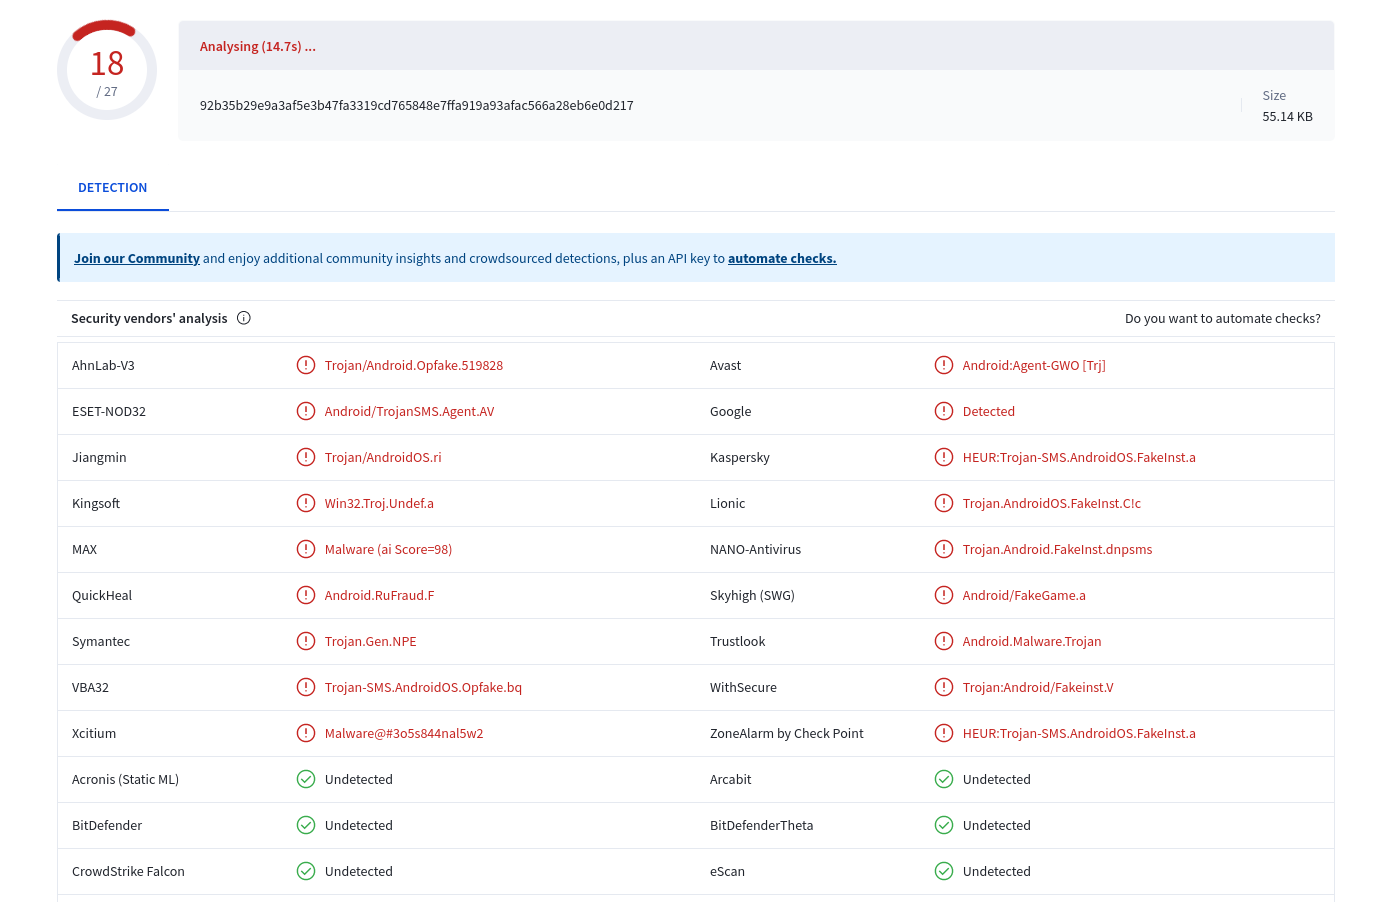
\includegraphics[width=0.8\textwidth]{visuals/virustotal.png}
      \caption{Procesul de scanare a unui fișier cu VirusTotal}
      \label{fig:vt_scan}
\end{figure}
\section{Hybrid Analysis}
Hybrid Analysis\cite{hybridanalysis} este un serviciu gratuit de analiză malware.
Utilizând acest serviciu, utilizatorii pot trimite fișiere pentru o analiză statică și dinamică detaliată.
Sistemul de analiză implicit suportă fișiere executabile, office, pdf, apk, jar și altele.
Acesta folosește analiză statică, analiză dinamică prin sandboxing și rezultatele antivirusului MetaDefender\cite{metadefener}.
\begin{figure}[H]
      \centering
      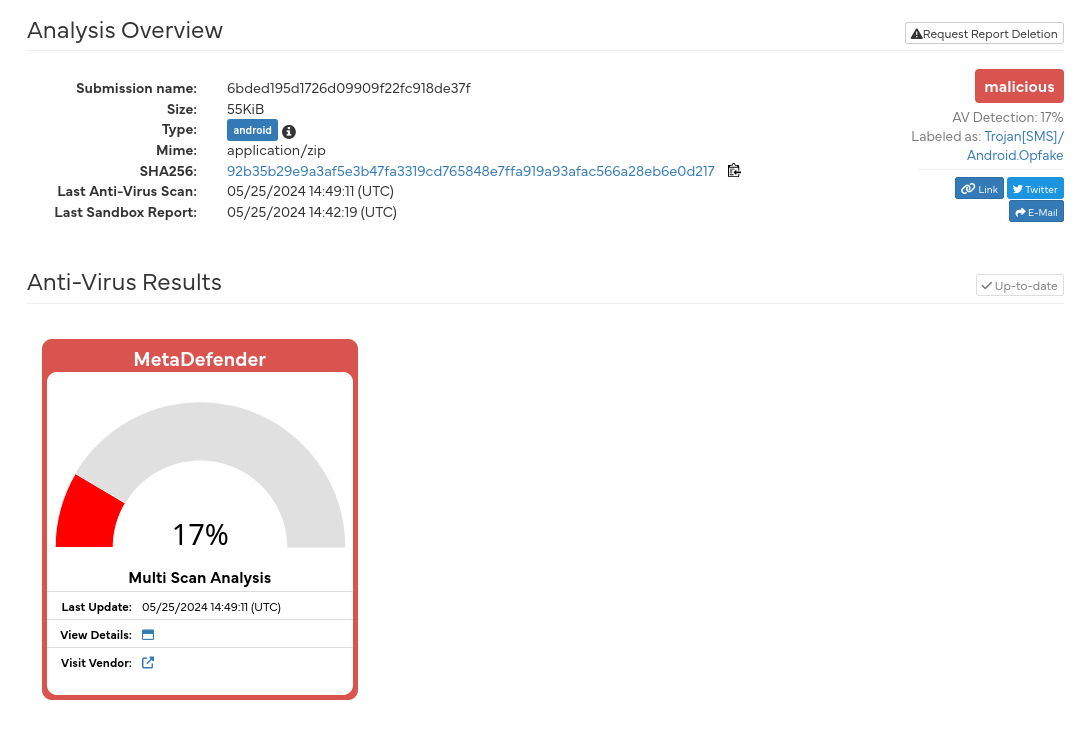
\includegraphics[width=0.8\textwidth]{visuals/hybrid_analysis.png}
      \caption{Rezultatele analizei unui fișier cu Hybrid Analysis}
      \label{fig:hybrid_analysis_result}
\end{figure}
\section{Jotti's Malware Scan}
Jotti's Malware Scan\cite{jotti} este un serviciu similar celor de mai sus,
care permite scanarea folosind produsele a 14 vendori populari de antiviruși, și căutarea rezultatelor scanarării fișierelor după hash.
\begin{figure}[H]
      \centering
      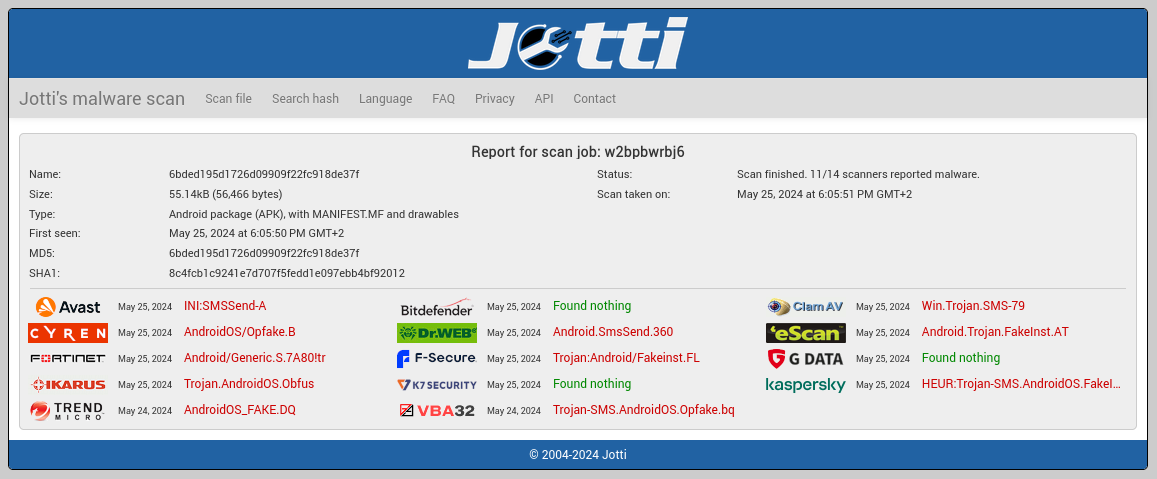
\includegraphics[width=0.8\textwidth]{visuals/jotti.png}
      \caption{Rezultatele analizei unui fișier cu Jotti's Malware Scan}
      \label{fig:jotti_result}
\end{figure}
\section{Comparație}
În \cref{tab:comparare_servicii} sunt comparate caracteristicile de analiză statică și căutare a serviciilor menționate anterior.
Pentru referință vor fi folosite următoarele:
\begin{enumerate}
      \item \textbf{Scanare proprie} - Algoritm propriu pentru analiză statică a fișierelor APK și nu doar grupare a rezultatelor vendorilor third-party.
      \item \textbf{Durată} - Durata medie de analiză a unui fișier APK în secunde. Metrica a fost măsurată folosind 5 fișiere scanate consecutiv de 3 ori.
      \item \textbf{Căutare hash} - Căutăre a rezultatelor scanării unui fișier după hash.
      \item \textbf{Căutare conținut} - Oferă posibilitatea interogării daca o secvență de octeți se consideră malware.
\end{enumerate}
\begin{table}[ht]
      \centering
      \begin{tabular}{lcccc}
            \toprule
            Caracteristică   & Serviciul meu & VirusTotal   & Hybrid Analysis & Jotti's Malware Scan \\
            \midrule
            Scanare proprie  & $\checkmark$  & -            & $\checkmark$    & -                    \\
            Durată           & 3.3           & 86.2         & 62.4            & 19.1                 \\
            Căutare hash     & $\checkmark$  & $\checkmark$ & $\checkmark$    & $\checkmark$         \\
            Căutare conținut & -             & -            & $\checkmark$    & -                    \\
            \bottomrule
      \end{tabular}
      \caption{Compararea caracteristicilor de analiză statică și căutare a serviciilor}
      \label{tab:comparare_servicii}
\end{table}

\chapter{Fundamentare teoretică}
\section{Android}
Android este un sistem de operare open source complet cu cod sursă personalizabil
care poate fi portat pe aproape orice dispozitiv, și cu documentație publică disponibilă
pentru toată lumea la \textit{source.android.com} pentru dispozitive mobile, condus de Google\cite{android-source}.
Platforma Open System Android (AOSP) este un cod sursă Android disponibil public și modificabil.
\begin{figure}[H]
      \centering
      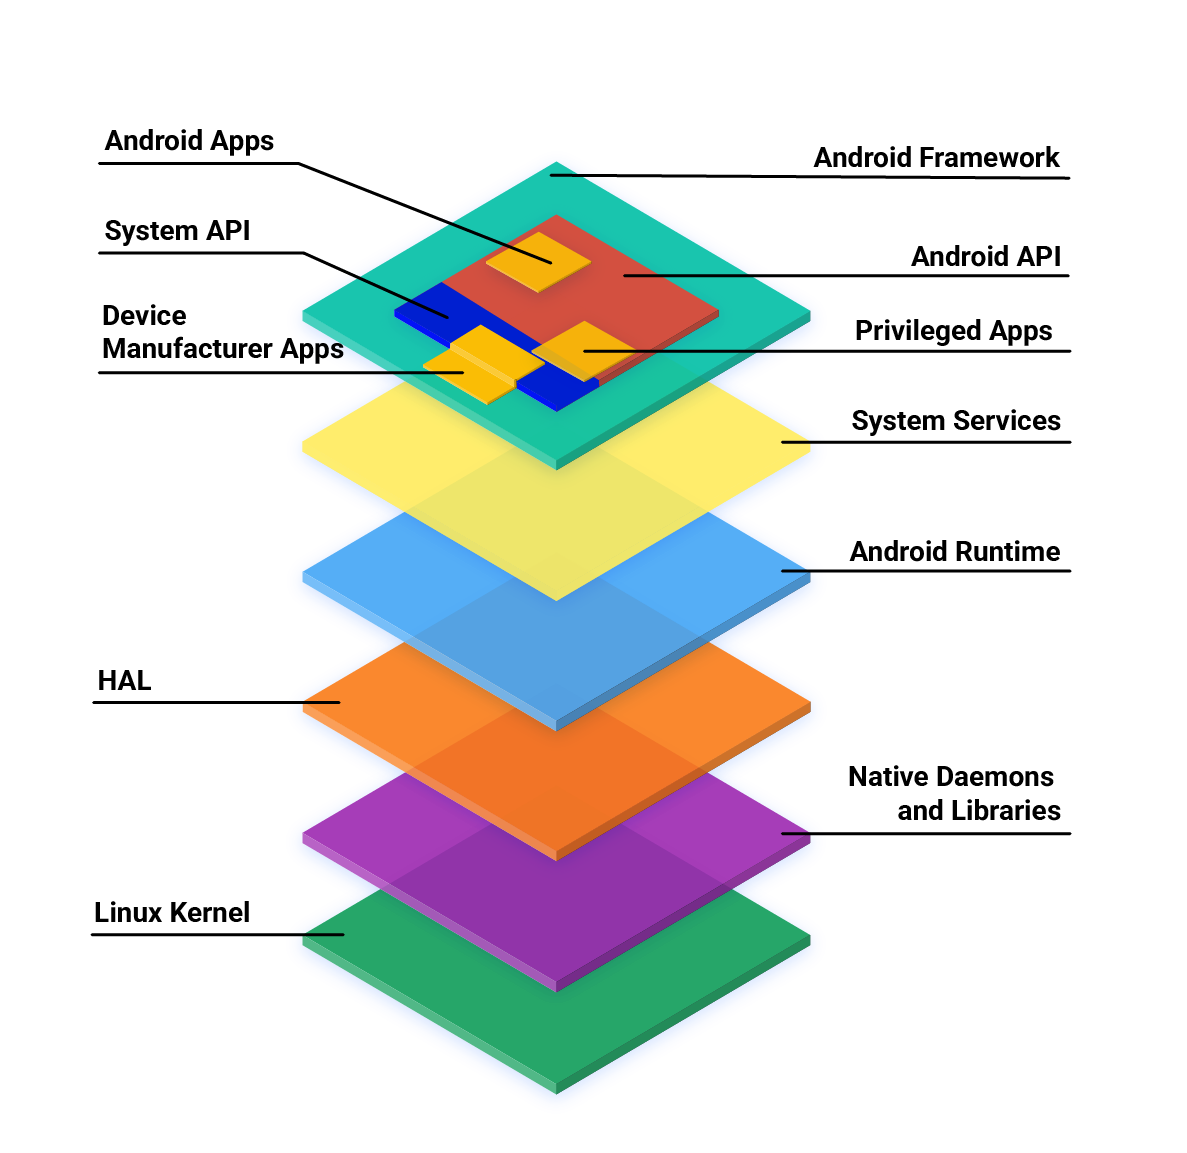
\includegraphics[width=0.8\textwidth]{visuals/android_stack.png}
      \caption{AOSP software stack architecture \cite{android-architecture}}
      \label{fig:android_stack}
\end{figure}
\subsection{Aplicații}
Aplicațiile Android pot fi scrise folosind Kotlin, limbajul de programare Java și limbajele C++.
Instrumentele SDK Android compilează codul împreună cu orice fișiere de date și resurse într-un APK sau un Android App Bundle.\cite{android-application-fundamentals}

Un pachet Android, care este un fișier de arhivă cu extensia \textit{.apk},
conține fișierele unei aplicații Android necesare la rulare și este fișierul pe care dispozitivele cu Android îl folosesc pentru a instala aplicația.\cite{android-application-fundamentals}

\subsection{Permisiuni}
Permisiunile aplicațiilor ajută la protejarea confidențialității utilizatorilor prin restricționarea accesului la următoarele:
\begin{itemize}
      \item Date restricționate, cum ar fi starea sistemului și informațiile de contact ale utilizatorilor
      \item Acțiuni restricționate, cum ar fi conectarea la un dispozitiv împerecheat și înregistrarea audio
\end{itemize}

Tipul fiecărei permisiuni indică domeniul datelor restricționate la care aplicația poate avea acces și domeniul acțiunilor restricționate
pe care aceasta poate efectua atunci când sistemul este acordată.\cite{android-permissions}

\subsection{Fișierul manifest}
Înainte ca sistemul Android să poată porni o componentă a aplicației, acesta trebuie să știe că acea componentă există citind fișierul manifest al aplicației,
\textit{AndroidManifest.xml}. Aplicația declară toate componentele și orice permisiuni de de care are nevoie,
cum ar fi accesul la internet sau accesul de citire la contactele utilizatorului sale în acest fișier,
care se află la rădăcina directorului proiectului aplicației.\cite{android-application-fundamentals}

\subsection{Android Runtime și Dalvik}
Android runtime (ART) este mediul de execuție utilizat de aplicații și unele servicii de sistem pe Android.
Acestea execută formatul Dalvik executable (DEX) și specificația bytecode DEX.\cite{android-runtime}

Dalvik Executable este un format de fișier binar care conține codul executabil al programului Android.
Acesta este bazat pe regiștri și poate fi ușor decompilat pentru a parcurge instrucțiunile fiecărei metode din fiecare clasă a aplicației.
Instrucțiunile constituie o secvență între 2 și 10 octeți, fiecare conține câte un opcode (primul octet) și un număr variabil de argumente fie regiștri, constante sau indecși din tabelele de identificatori.

\section{Rust}
Rust\cite{rustlang} este un limbaj de programare axat pe siguranță, viteză și concurență, extrem de rapid și eficient din punct de vedere al memoriei care se potrivește pentru servicii unde performanța este un factor critic.

Sistemul de tipuri bogat al limbajului și modelul de ownership garantează siguranța memoriei și a firelor de execuție — permițând eliminarea multor clase de erori în timpul compilării.

\section{Tensorflow}
Tensorflow\cite{tensorflow2015-whitepaper} este o bibliotecă open-source de \textit{machine learning} dezvoltată de echipa Google Brain,
care oferă un set larg de instrumente high-level pentru construirea, antrenarea și inferența modelelor de inteligență artificială.
Acesta este implementant în limbajul C++ și oferă API-uri pentru diferite limbaje cum ar fi Python și Javascript.

\section{Axum}
Axum\cite{axum-framework} este un framework pentru aplicații web care se concentrează pe ergonomie și modularitate.
Acesta permite dezvoltarea rapidă a REST-API-urilor folosind un model de programare asincron, bazat pe următoarele caracteristici cheie:
\begin{itemize}
      \item Redirecționarea cererilor HTTP către handlere cu un API fără macro-instrucțiuni.
      \item Parsarea declarativă a cererilor folosind extractori.
      \item Model simplu și previzibil de gestionare a erorilor.
      \item Generarea răspunsurilor fără cod reduntant.
\end{itemize}


\section{React}
React\cite{react} este o bibliotecă JavaScript pentru construirea interfețelor de utilizator. Avantajele bibliotecii sunt:
\begin{itemize}
      \item Paradigmă declarativă care face ușoară crearea de UI-uri interactive, iar codul să fie mai predictibil și mai ușor de înțeles.
      \item Componente reutilizabile care permit definirea unei componente și utilizarea acesteia oriunde în aplicație.
\end{itemize}


\section{MongoDB}
MongoDB\cite{mongodb} este o bază de date NoSQL orientată pe documente cu o serie de avantaje:
\begin{itemize}
      \item Structura flexibilă a documentelor.
      \item Interogare simplă a datelor.
      \item Framework de agregare robust.
      \item Scalare orizontală.
\end{itemize}

Documentele sunt structurate într-un format similar JSON numit BSON (Binary JSON),
care reprezintă o serializare binară a documentelor, cu anumite extensii care permit utilizarea unor structuri de date mai complexe
cum ar fi date calendaristice.

MongoDB este o alegere populară pentru aplicații cu potențial de scalabiliate și volatilitate a datelor.


\chapter{Soluția propusă}


\chapter{Implementare}
În acest capitol sunt prezentate detaliile de implementare ale tuturor unităților sistemului.

\section{Frontend}
Interfața web este entry-point-ul pentru utilizatorii aplicației.
Elaborată folosind framework-ul React\cite{react}, aceasta conține:
\begin{itemize}
      \item Câmp pentru încărcare fișiere
      \item Buton upload fișiere
      \item Câmp pentru introducere hash SHA-256
      \item Buton pentru verificare hash
\end{itemize}
După trimiterea fișierelor către backend, interfața va iniția animația unui spinner de încărcare
până când nu e primit răspunsul de la server.
Răspunsul va fi afișat sub forma unei liste cartonașe care conțin:
\begin{itemize}
      \item Numele fișierului
      \item Hash-ul SHA-256
      \item Categorie prezisă
      \item Probabilitatea categoriei
\end{itemize}

Aceeași procedură va fi inițiată în urma trimiterii unui hash, răspunsul de la server fiind similar.

\section{REST API}
API-ul backend este realizat folosind framework-ul axum\cite{axum-framework}.
Este un API asincron care oferă următoarele rute:
\begin{itemize}
      \item \texttt{POST /scan} - Acceptă unul sau mai multe fișiere APK și returnează predicțiile în formatul JSON ca în \cref{fig:api_response}
      \item \texttt{GET /query/:hash} - Returnează predicția pentru un fișier APK după hash-ul SHA256, răspunsul e similar cu cel de la \texttt{POST /scan} doar că pentru un singur fișier.
\end{itemize}
\begin{figure}[H]
      \centering
      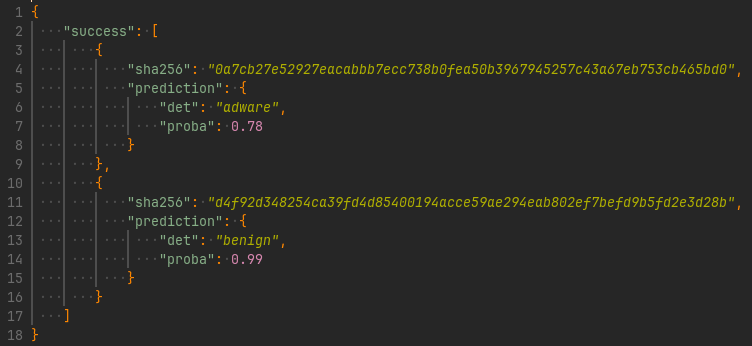
\includegraphics[width=0.8\textwidth]{visuals/api_response.png}
      \caption{Exemplu de răspuns al API-ului}
      \label{fig:api_response}
\end{figure}

\subsection{Scanare}
În momentul încărcării fișierelor, 
se va face o prefiltrare pentru a lăsa doar fișierele al cărui conținut începe 
cu \texttt{b"PK"} (începutul headerului unui fișier ZIP),
pentru a preveni încercarea de a scana fișiere ce nu sunt APK-uri.

Înainte de scanare se calculează hash-ul SHA256 și se caută în baza de date MongoDB\cite{mongodb}.
Dacă fișierul a fost scanat anterior, se va returna rezultatul salvat în baza de date.
În caz contrar se va face predicția pe fișier folosind biblioteca de extragere a datelor
și modelul încărcat folosind binding-urile Tensorflow pentru Rust. 
Rezultatele scanării sunt salvate în baza de date pentru a fi folosite ulterior,
iar răspunsul este trimis înapoi către client.

În caz că se încarcă mai multe fișiere odată, procesul va fi optimizat să facă căutare în
baza de date cu mai multe hash-uri odată, iar extragerea de date va fi paralelizată folosind
biblioteca \textit{rayon}\cite{rayon} care facilitează conversia calculelor 
secvențiale în calcule paralele, printr-un API simplu și intuitiv. Scanarea va fi aplicată
doar fișierelor care nu au fost găsite în baza de date.


\section{Extragere de date}
Biblioteca de extragere a datelor realizată în cadrul lucrării expune funcția:
\begin{lstlisting}[language=Rust]
parse<R: Read + Seek>(apk: R) -> Result<Apk, ApkParseError>
\end{lstlisting}
Aceasta acceptă un buffer de memorie care reprezintă arhiva APK și returnează un rezultat
care conține structura de date \textit{Apk} (\cref{fig:apk_struct}) sau o eroare de parsare \textit{ApkParseError}.
\begin{figure}[H]
      \centering
      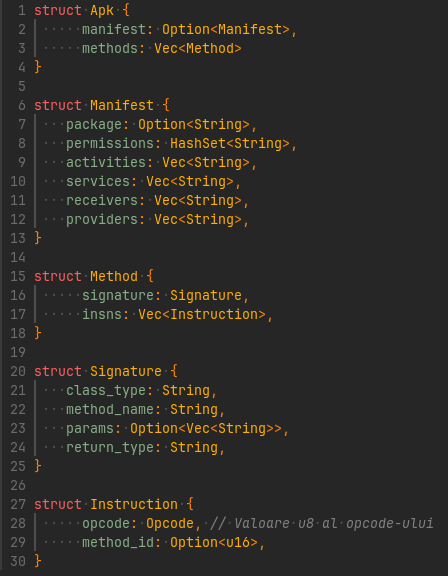
\includegraphics[width=0.8\textwidth]{visuals/structs.png}
      \caption{Structura de date Apk}
      \label{fig:apk_struct}
\end{figure}

În momentul apelării, se vor parcurge fișierele din arhivă pentru a găsi:
\begin{enumerate}
      \item Fișierul \textit{AndroidManifest.xml} al aplicației care declară componentele și permisiunile necesare.
      \item Orice fișier binar al cărui header corespunde cu \texttt{DEX\_FILE\_MAGIC}\cite{dex-format},
            fiind considerat un fișier Dalvik Executable cu cod al aplicației.
\end{enumerate}

\subsection{Componente și permisiuni}
Întrucât fișierul \textit{AndroidManifest.xml} din cadrul arhivei nu este un fișier XML standard,
ci o reprezentare serializată binar a documentului, se folosește biblioteca \textit{abxmldecoder}\cite{abxmldecoder}
pentru parcurgerea node-urilor și parsarea informației utile.

Componentele și denumirea pachetului sunt salvate pentru a fi folosite ulterior în sortarea metodelor din fișierele DEX. Există 4 tipuri de componente:
\begin{itemize}
      \item Activități - Interfețe grafice cu care utilizatorul interacționează.
      \item Servicii - Rulează în fundal și nu au interfață grafică.
      \item Receivers - Răspund la anumite evenimente cum ar fi primirea unui SMS.
      \item Providers - Oferă acces la datele aplicației.
\end{itemize}

Permisiunile sunt extrase din nodurile \textit{uses-permission} și salvate într-un \textit{HashSet$<$String$>$}.

\subsection{Bytecode}
Un APK poate avea mai multe fișiere DEX, de obicei se găsesc în directorul root al arhivei și sunt denumite \textit{classes.dex}, \textit{classes2.dex}, etc.
Dat fiind faptul că aceasta este doar o convenție de denumire, un atacator poate liber ascunde cod executabil în alte directoare sau sub alt nume,
de aceea sunt parcurse și verificate cu o expresie regulată \texttt{b"6465780A3033[35-39]00"} (Validează versiunile 35-39) header-ele tuturor fișierelor din arhivă.
\begin{figure}[H]
      \centering
      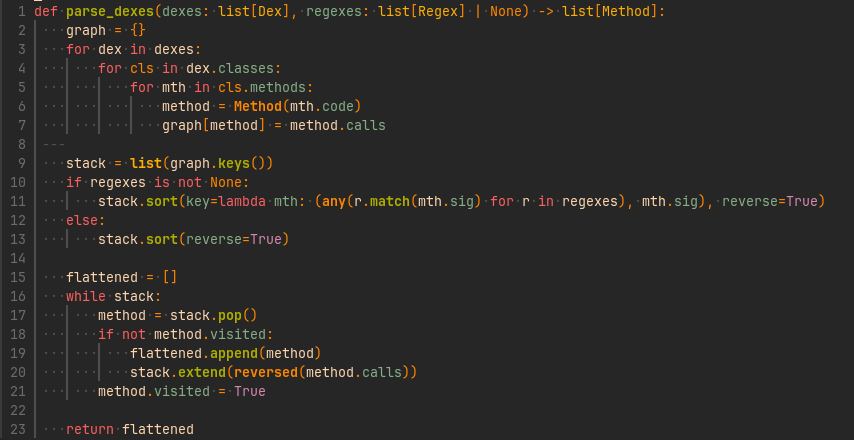
\includegraphics[width=0.8\textwidth]{visuals/method_extraction.png}
      \caption{Algoritmul de parsare a metodelor (Abstractizat)}
      \label{fig:bytecode_parsing}
\end{figure}

Conform algoritmului, sunt parcurse toate metodele din fișierele DEX pentru a se construi un Control Flow Graph.
Graph-ul este aplatizat și sortat în așa manieră ca metodele din clasele declarate ca componente în Manifest să fie parcurse primele:
\begin{enumerate}
      \item \textbf{Major Order} - Clasa este declarată în AndroidManifest.xml ca componentă
      \item \textbf{Minor Order} - Signatura metodei, ex. \texttt{Lcom/test/MAct;->v(I;)V}
\end{enumerate}

După această sortare graph-ul este reparcurs folosind Depth-First Search\cite{depth-first-search}
pentru a se construi vectorul de metode normalizat utilizat* la clasificare, similar cu cel din \cref{fig:f-droid-json}.
Codul sursă este scris în Rust pentru a beneficia de performanța și siguranța limbajului,
iar în scopuri demonstrative este o inclusă o versiune abstractizată a algoritmului de procesare DEX (\cref{fig:bytecode_parsing}).
\begin{figure}[H]
      \centering
      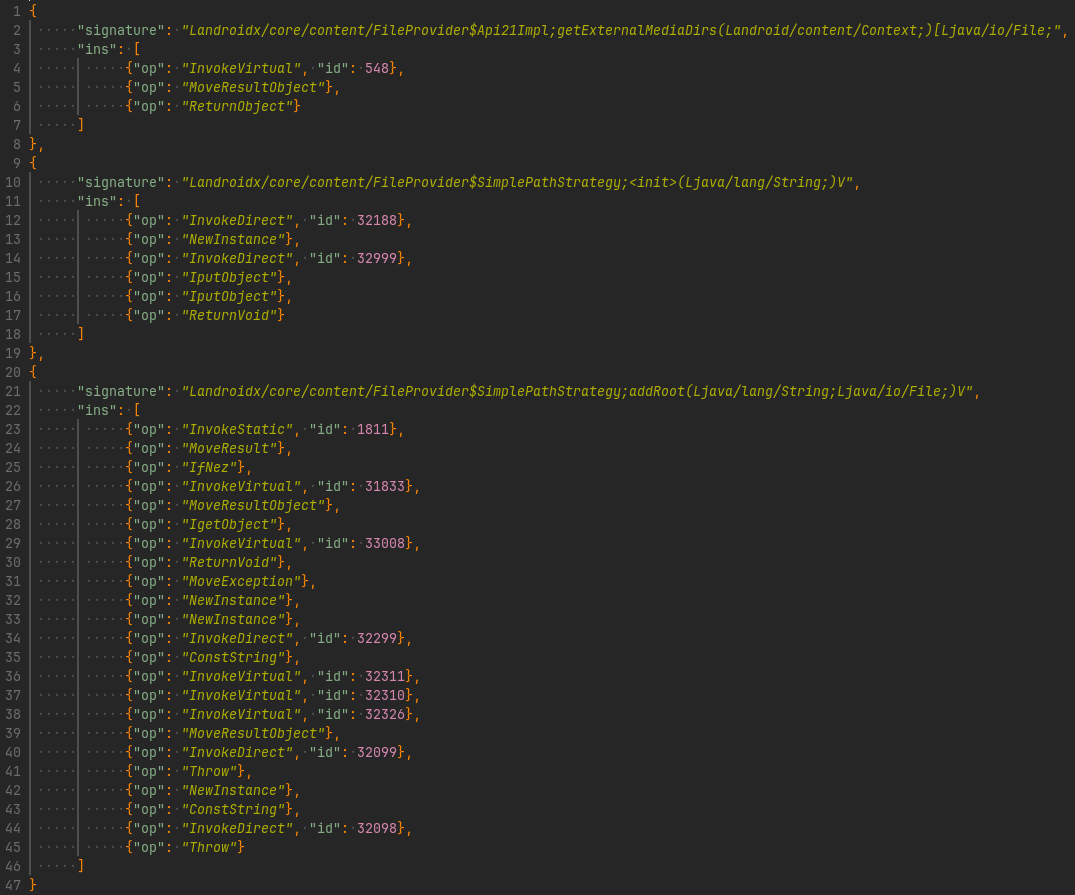
\includegraphics[width=0.8\textwidth]{visuals/methods_json.png}
      \caption{Exemplu de secvență de metode extrasă din aplicația F-Droid\cite{f-droid} (JSON)}
      \label{fig:f-droid-json}
\end{figure}

\subsection{Preprocesare}
Dat fiind faptul că biblioteca de extragere a datelor returnează o instanță a structurii \textit{Apk},
și modelele machine learning nu înțeleg structuri de date complexe,
este necesară transformarea \textit{Apk}-ului într-un input care poate fi folosit de model.
Această parte nu este implementată în bibliotecă, ci este un modul separat din aplicația web.

Modelul nu poate accepta set-ul de permisiuni ca un array de string-uri.
Acesta este convertit într-un vector binar de dimensiunea 50,
unde fiecare poziție înseamnă prezența sau absența unei permisiuni în \textit{AndroidManifest.xml}:
\begin{itemize}
      \item 1 - Permisiunea este declarată
      \item 0 - Permisiunea nu este declarată
\end{itemize}
Aplicațiile Android pot declara sute de permisiuni, dar în practică unele permisiuni sunt foarte rar întâlnite și nu sunt relevante.
Pentru eliminarea permisiunilor redundante a fost folosit un clasificator Random Forest\cite{breiman2001random}\cite{Khariwal2021}.
Setul total de 368 de permisiuni întâlnite în dataset, a fost redus, folosind codul Python din \cref{fig:rf_train}, la 50 de permisiuni cele mai relevante (\cref{fig:top50}), top 5 fiind:
\begin{enumerate}
      \item \texttt{SEND\_SMS} - Permite trimiterea mesajelor SMS.
      \item \texttt{RECEIVE\_SMS} - Permite citirea mesajelor SMS.
      \item \texttt{MOUNT\_UNMOUNT\_FILESYSTEMS} - Permite montarea și demontarea sistemului de fișiere.
      \item \texttt{READ\_PHONE\_STATE} - Permite accesul (read-only) la starea telefonului, inclusiv la informațiile actuale ale rețelei celulare, la starea oricăror apeluri în curs și la o listă a oricăror conturi de telefon înregistrate pe dispozitiv.
      \item \texttt{ACCESS\_WIFI\_STATE} - Permite accesarea informațiilor despre rețelele Wi-Fi.
\end{enumerate}
\begin{figure}[H]
      \centering
      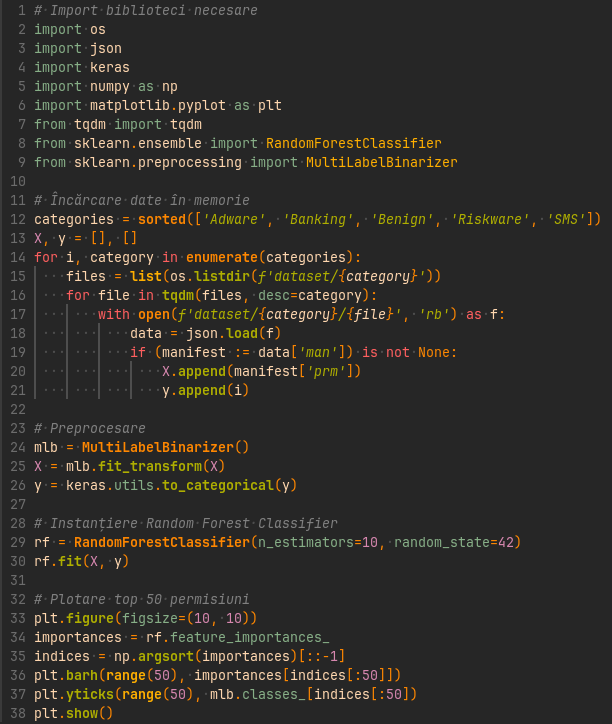
\includegraphics[width=0.8\textwidth]{visuals/rf_train.png}
      \caption{Selectarea celor mai importante 50 de permisiuni}
      \label{fig:rf_train}
\end{figure}
\begin{figure}[H]
      \centering
      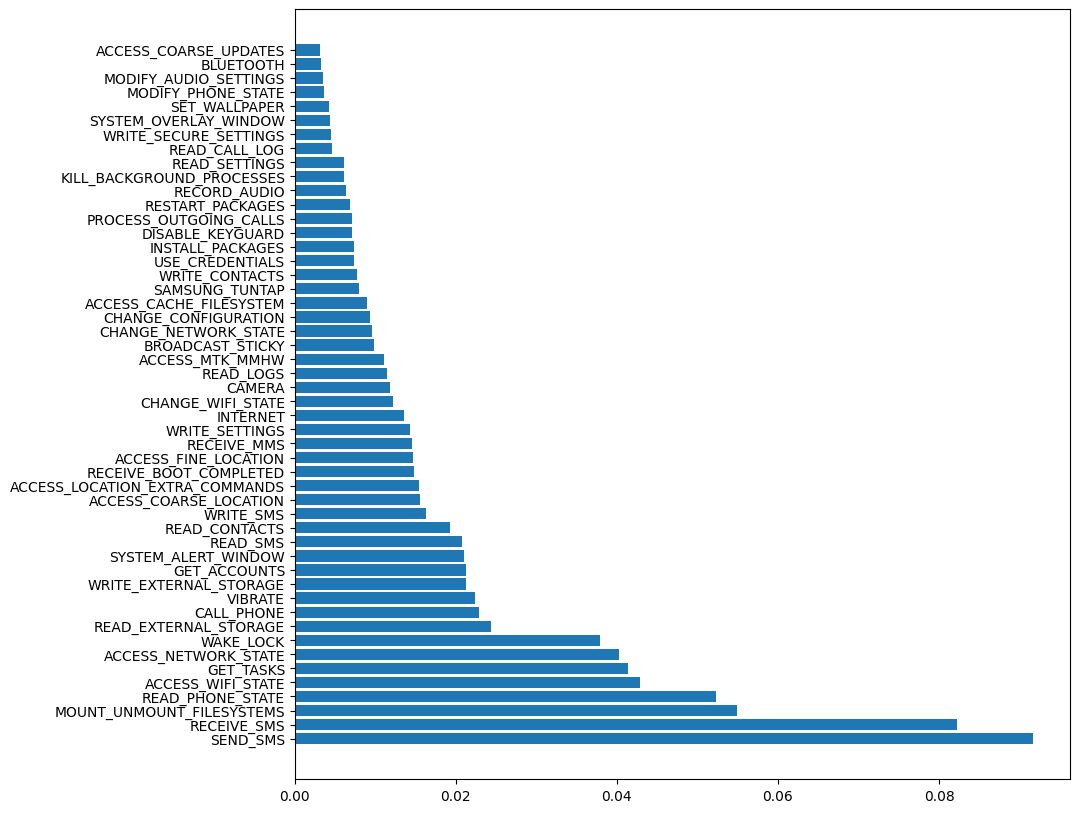
\includegraphics[width=0.8\textwidth]{visuals/top50.png}
      \caption{Top 50 cele mai importante permisiuni}
      \label{fig:top50}
\end{figure}

La fel ca și cu permisiunile, metodele nu pot fi transmise direct. Vectorul de metode este convertit în doi vectori separați:
\begin{itemize}
      \item \textbf{Opcode Vector} - Secvența de opcode-uri concatenată a tuturor metodelor.
      \item \textbf{Indices Vector} - Vector de indici [start, end] care delimitează metodele în \textbf{Opcode Vector}.
\end{itemize}
Pe lângă aceasta mai e de menționat că vectorii vor fi truncați astfel încât ultimul index de start de metodă
să fie sub valoarea 512000 (\cref{fig:cap}) pentru a preveni supraîncărcarea memoriei.
\begin{figure}
      \centering
      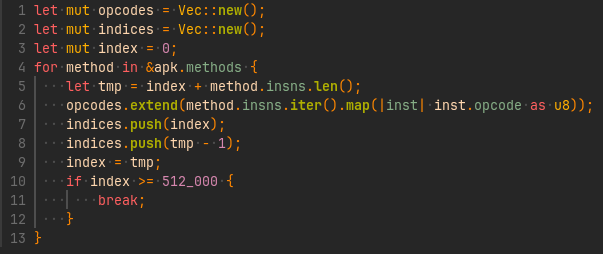
\includegraphics[width=0.8\textwidth]{visuals/cap.png}
      \caption{Truncarea secvenței bytecode pentru un APK}
      \label{fig:cap}
\end{figure}

Astfel vom avea un vector de dimensiune fixă 50 cu valori 0, 1 pentru permisiuni
și doi vectori de dimensiune variabilă pentru bytecode-ul aplicației.

\subsection{Testare}
Pentru asigurarea corectitudinii parsării APK-urilor, a fost elaborată o suită de teste unitare
folosind biblioteca standard din Rust.
În total au fost scrie 10 teste unitare:
\begin{enumerate}
      \item \verb|dex::instruction::tests::test_empty_bytecode|
      \item \verb|dex::instruction::tests::test_bad_opcode|
      \item \verb|dex::instruction::tests::test_invoke_args|
      \item \verb|dex::instruction::tests::test_too_short|
      \item \verb|dex::instruction::tests::test_valid_opcode|
      \item \verb|dex::tests::test_hello_world|
      \item \verb|dex::tests::test_call_graph|
      \item \verb|manifest::tests::test_parse_a|
      \item \verb|manifest::tests::test_parse_b|
      \item \verb|manifest::tests::test_parse_c|
\end{enumerate}

Testele 1-5 asigură corectitudinea parsării instrucțiunilor individuale din cadrul unei secvențe de octeți.

Testele 6-7 verifică ordinea și integritatea metodelor extrase din fișiere DEX.
Fișierele DEX au fost generate manual prin compilarea de cod Java 
și conversia rezultatului binar în format DEX folosind instrumentul de linie de comandă \textit{d8}\cite{d8}.

Testele 8-10 asigură corectitudinea parsării componentelor și permisiunilor din fișiere \textit{AndroidManifest.xml}.
Fișierele au fost obținute prin build-area manuală a unor proiecte Android simple pentru a obține fișiere .apk,
care au fost dezarhivate pentru a extrage \textit{AndroidManifest.xml} în formatul lor binar.

\section{Clasificare}
\subsection{Dataset}
În cadrul acestei lucrări, a fost folosit datasetul CICMalDroid 2020 \cite{cicmaldroid0, cicmaldroid1} pentru antrenarea și testarea modelului.
Setul de date conține 17341 de aplicații Android colectate în perioada Decembrie 2017 - Decembrie 2018 din cinci categorii:
\begin{itemize}
      \item \textbf{Adware} - Afișează material publicitar nesolicitat.
      \item \textbf{Banking} - Obține acces la conturile bancare online ale utilizatorului,
            imitând aplicațiile bancare originale sau interfața web bancară.
            Majoritatea sunt concepute pentru a se infiltra în dispozitive și fura detalii sensibile,
            de exemplu, loginul și parola contului bancar și pentru a trimite informațiile
            furate către un server de comandă și control (C\&C).
      \item \textbf{SMS} - Exploatează serviciul SMS, pentru a trimite sau intercepta mesaje cu scopul
            răspândirii virusului și exfiltrării datelor.
      \item \textbf{Riskware} - Pot cauza daune dacă utilizatorii rău intenționați le exploatează.
            Se poate transforma în orice altă formă de malware, cum ar fi Adware sau Ransomware,
            care extinde funcționalitățile instalând aplicații nou infectate.
      \item \textbf{Benign} - Aplicații care nu sunt rău intenționate.
\end{itemize}
După preprocesare, doar 16457 de aplicații au fost decompilate cu succes, rezultând numerele finale din \cref{fig:df_distro}.
\begin{figure}[H]
      \centering
      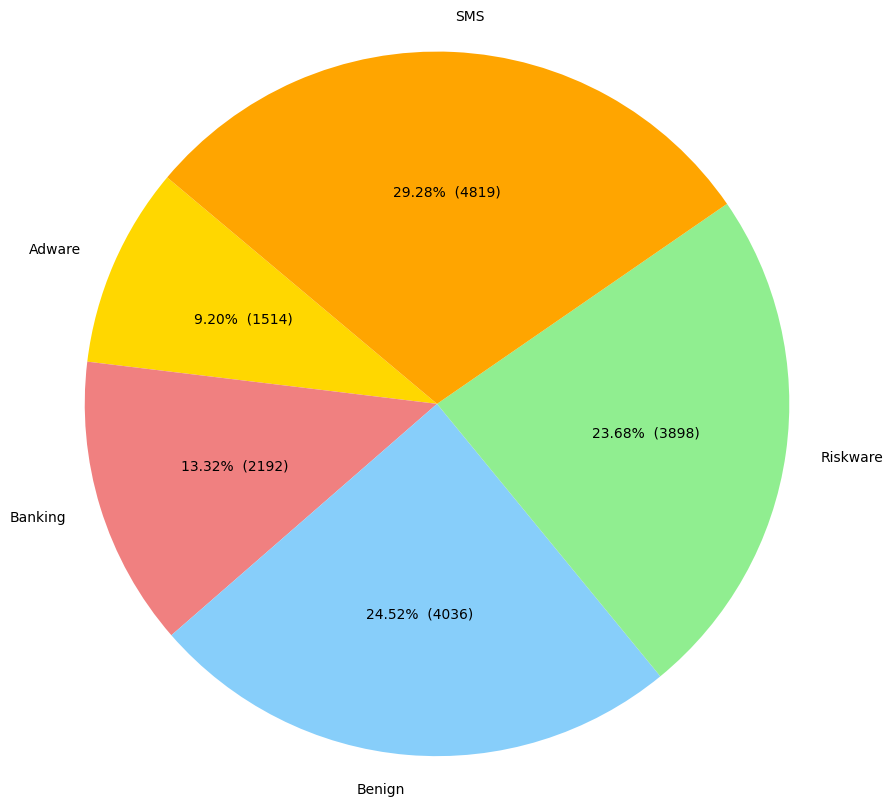
\includegraphics[width=0.8\textwidth]{visuals/df_distro.png}
      \caption{Distribuția finală a categoriilor în setul de date}
      \label{fig:df_distro}
\end{figure}
Pentru antrenare a fost folosit un subset de 80\% din date (din care 20\% pentru validare) și 20\% pentru testare.

\subsection{Model}
La implementării din lucrare stă arhitectură ierarhică de blocuri PerceiverIO\cite{jaegle2022perceiver}
a modelului Malceiver\cite{mclaughlin2022malceiver} care folosește 3 feature-uri la nivel de cod:
\begin{enumerate}
      \item $C$ - Caracteristicile locale la nivel de relat, ii între opcodes învecinați
      \item $M$ - Caracteristicile la nivel de metodă
      \item $g$ - Caracteristicile la nivel global
\end{enumerate}

\subsection{Nivel local}
Secvența de opcode-uri este trecută printr-un strat Embedding pentru a învăța reprezentările semantice a fiecărui opcode.
Acestor reprezentări le este aplicată o convoluție pentru a captura relațiile dintre opcode-uri și a comprima secvența\cite{hassani2022escaping}.

Astfel se obține o matrice de filtre convoluționale $C \in \mathbb{R}^{n \times c}$,
unde $n$ corespunde cu lungimea secvenței iar $c$ corespunde cu numărul de filtre convoluționale.
Aceasta este introdusă în primul bloc PerceiverIO care va returna matricea latentă pentru următorul bloc.

\subsection{Nivel de metodă}
Se calculează suma cumulată a matricii $C$, și se obține matricea $\hat{C} \in \mathbb{R}^{n \times c}$.
Apoi se calculează o sinteză a fiecărei metode folosind vectorul de indici $\mathcal{F}$ și matricea $\hat{C}$:
$$ M = \left( \frac{\widehat{C}_{e_f} - \widehat{C}_{s_f}}{e_f - s_f} \right), (s_f, e_f) \in \mathcal{F} $$
Prin aceasta se obține matricea $M \in \mathbb{R}^{F \times c}$, $F$ fiind numărul de metode din APK.
Matricea conține sinteze a tuturor metodelor, fiecare fiind normalizată folosind lungimea sa.
Se introduce matricea în al doilea bloc PerceiverIO care va returna matricea latentă pentru următorul bloc.

\subsection{Nivel global}
Se aplică Global Max-Pooling peste matricea $C$, și se obține un vector de caracteristici $g \in \mathbb{R}^{1 \times n}$ care reprezintă o sinteză globală bytecode-ului.
Se introduce în al treilea bloc PerceiverIO care va returna matricea latentă pentru concatenare cu output-ul de la Multi Layer Perceptron (MLP)\cite{haykin1994neural} al permisiunilor.

\begin{figure}[H]
      \centering
      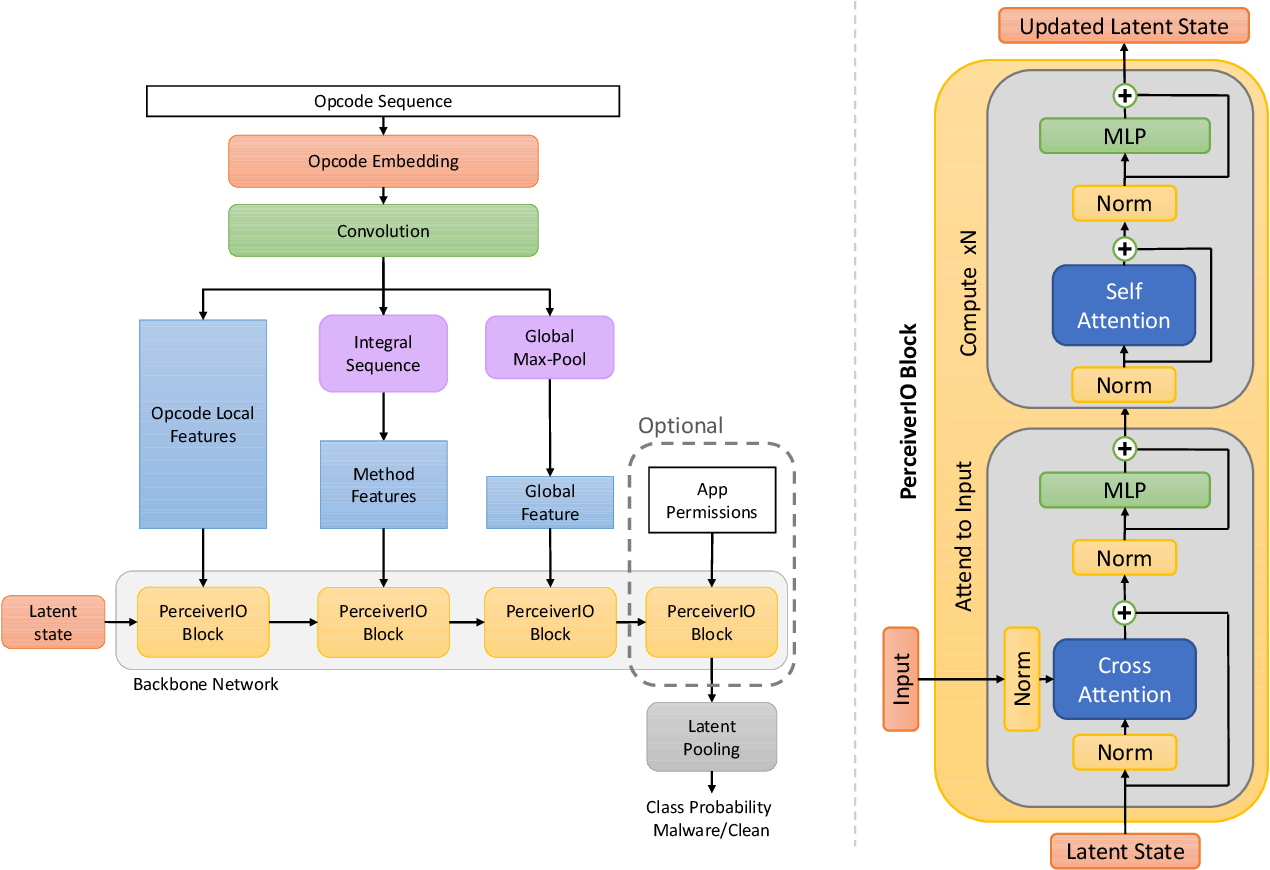
\includegraphics[width=0.8\textwidth]{visuals/malceiver.png}
      \caption{Arhitectura Rețelei Malceiver\cite{mclaughlin2022malceiver} (Figura 1) \textit{arXiv:2204.05994}, 2022. \href{https://doi.org/10.48550/arXiv.2204.05994}{doi:10.48550/arXiv.2204.05994}.}
      \label{fig:malceiver}
\end{figure}

\subsection{Permisiuni}
Una din deviațiile de la implementarea originală a modelului Malceiver din \cref{fig:malceiver} constă în abordarea diferită a permisiunilor.
În loc să fie folosit un strat Embedding și încă un bloc PerceiverIO, se folosește un simplu MLP,
rezultatul fiind concatenat cu matricea latentă finală la care s-a aplicat un Global Average Pooling.
În urma experimentării sa depistat că această concatenare a dat rezulate mai bune,
iar numărul de parametri a fost redus.

\subsection{Output}
Vectorul concatenat este unit cu un strat alcătuit din 5 neuroni corespunzători fiecărei categorii.
Funcția de activare folosită este \textit{sigmoid} pentru fiecare neuron, iar funcția de loss este \textit{Binary Crossentropy}.
Aceasta a fost o modificare minoră față de implementarea originală pentru a adapta modelul la clasificare multi-label în loc de binară.
Prin unirea tuturor blocurilor este obținut modelul final din \cref{fig:model} antrenat pe datasetul CICMalDroid 2020\cite{cicmaldroid0,cicmaldroid1}.

\begin{figure}[H]
      \centering
      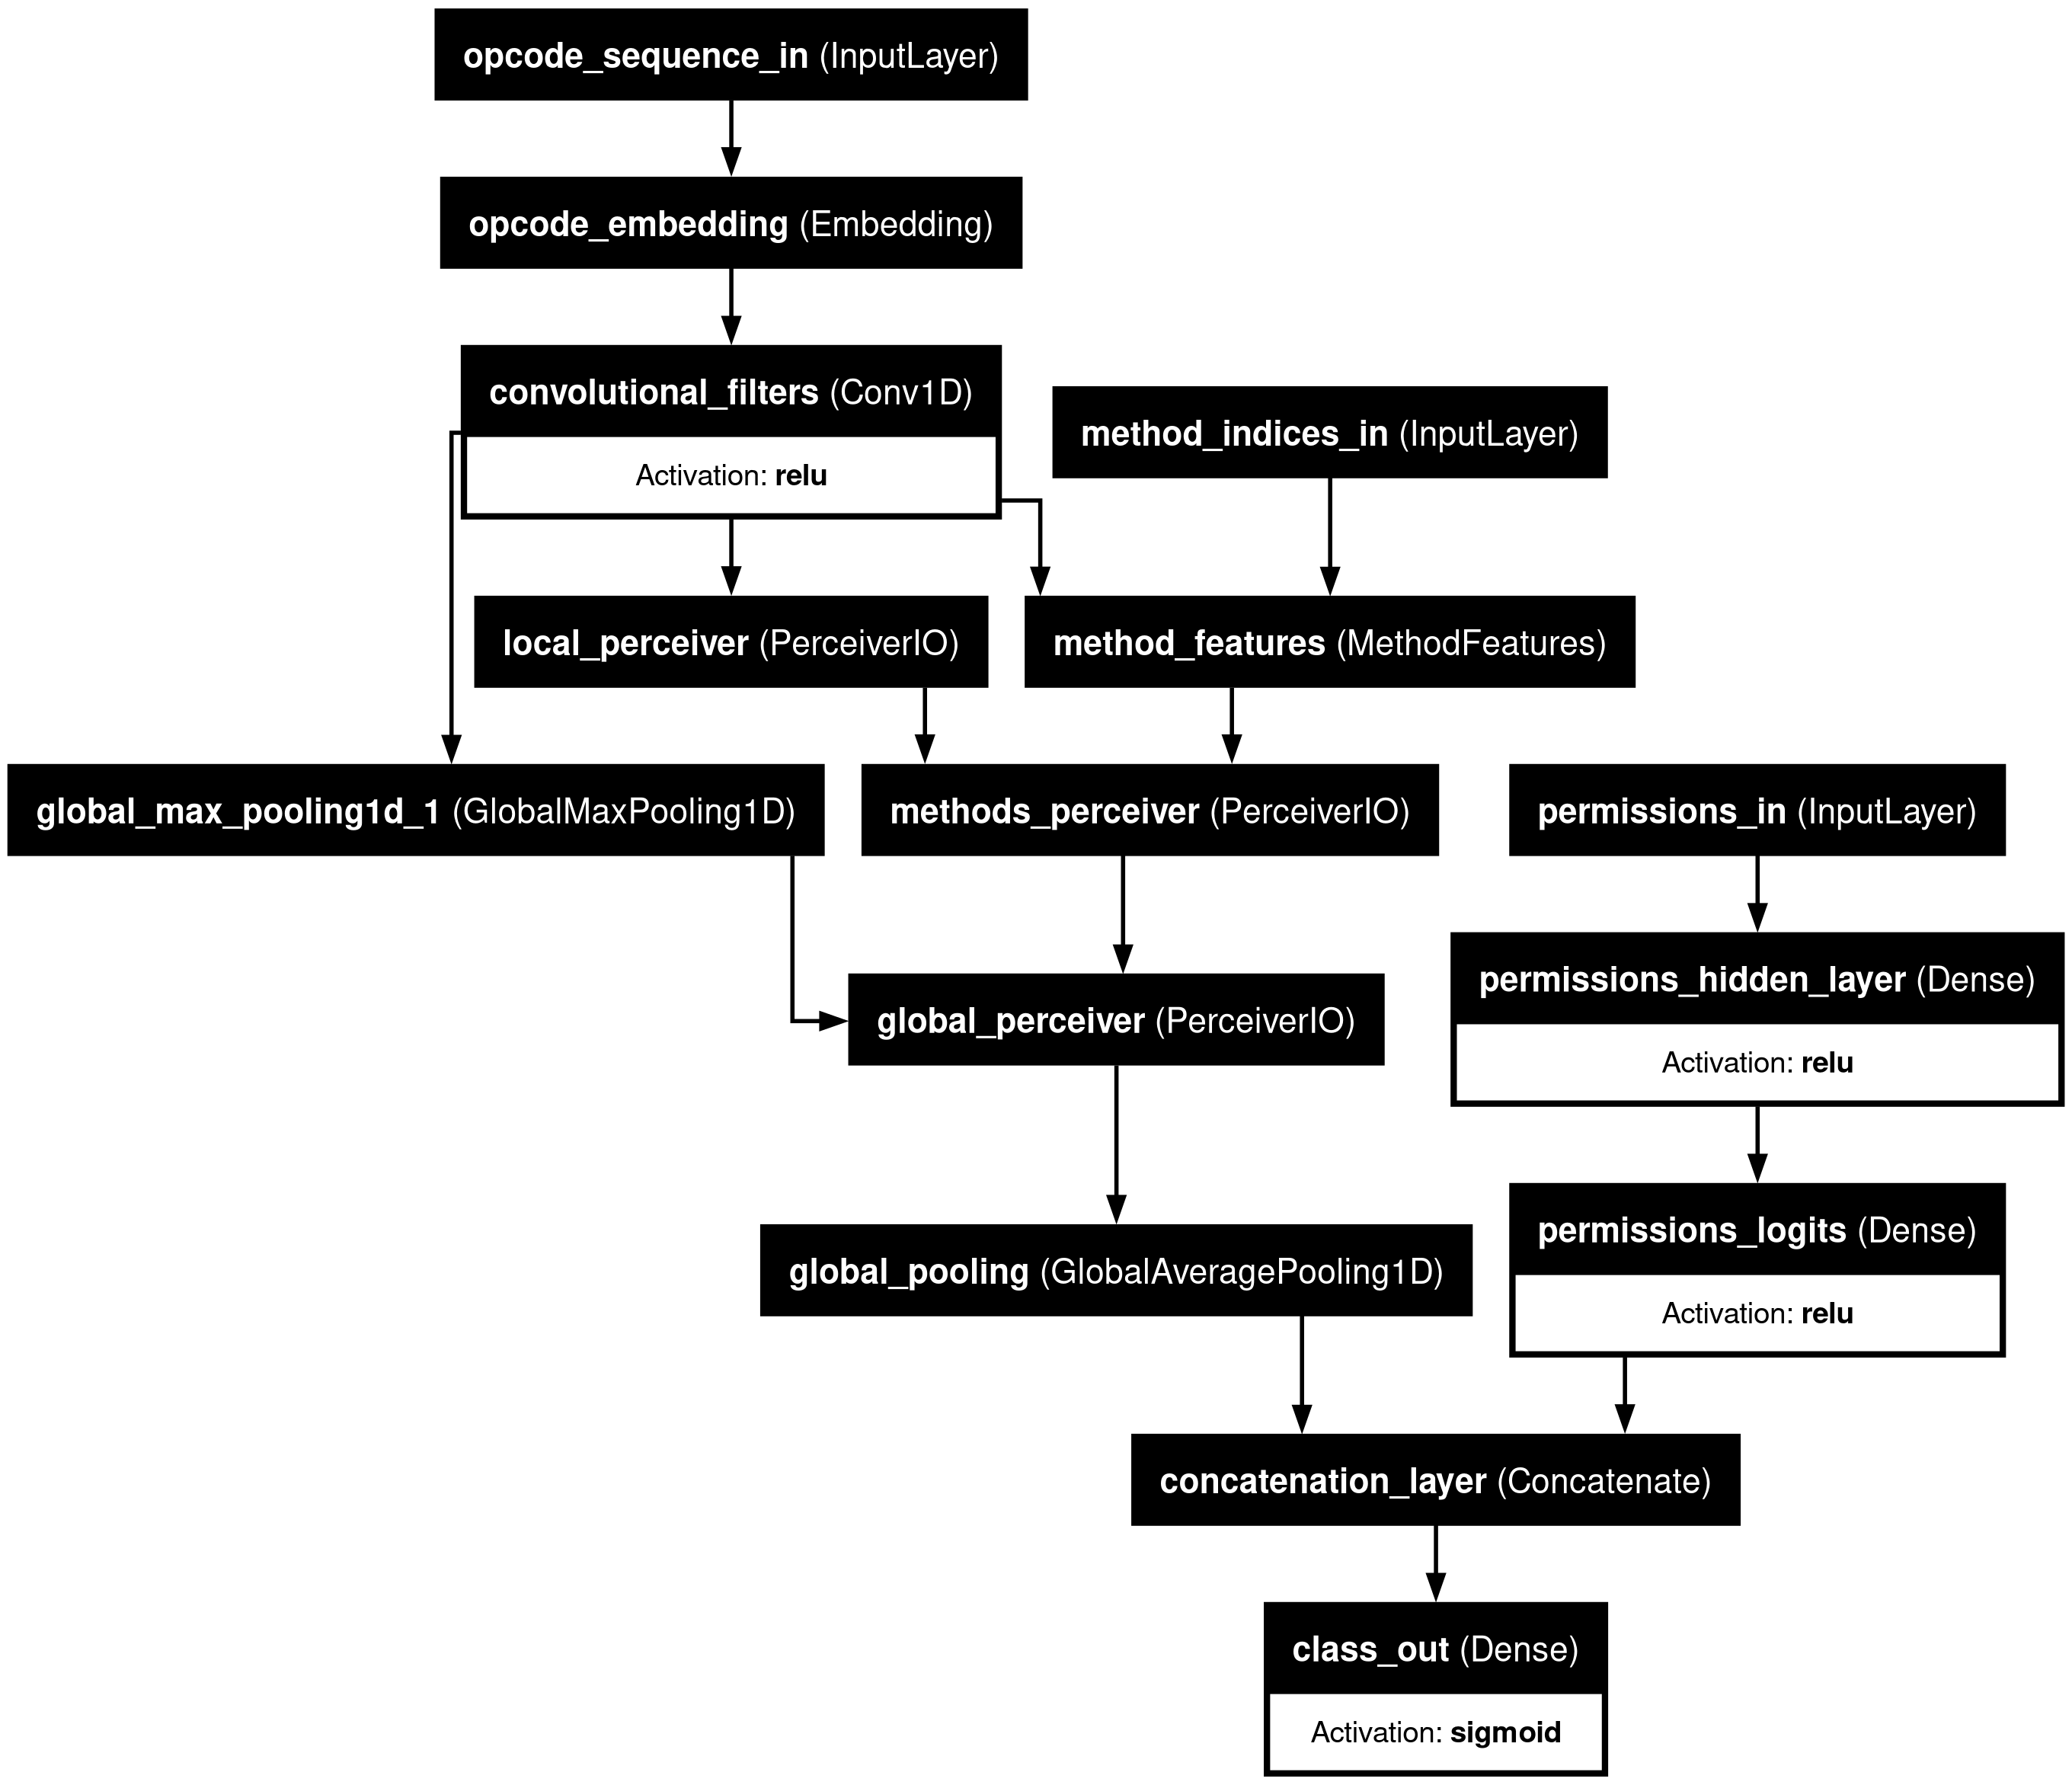
\includegraphics[width=0.8\textwidth]{visuals/model.png}
      \caption{Modelul final}
      \label{fig:model}
\end{figure}

\subsection{Antrenare}
Antrenarea a fost realizată folosind biblioteca Keras\cite{chollet2015keras} pentru Python.
Keras simplifică antrenarea modelului prin expunerea unor funcționalități precum callback-uri.
Astfel este posibilă o antrenare fără cod redundant și cu o structură clară ca în \cref{fig:train}.

Pentru a asigura obținerea celui mai performant model, a fost folosit callback-ul \textit{ModelCheckpoint}. 
\textit{ModelCheckpoint} salvează modelul/ponderile într-un fișier dacă metrica prestabilită este îmbunătățită.
În cazul modelului elaborat, metrica prestabilită a fost \textit{val\_accuracy} (acuratețea pe setul de validare).

Prevenirea overfitting-ului este realizată de callback-ul \textit{EarlyStopping}.
\textit{EarlyStopping} oprește antrenarea dacă metrica prestabilită (\textit{val\_accuracy}) nu se îmbunătățește într-un număr de epoci consecutiv,
5 în cazul modelului elaborat.


\begin{figure}[H]
      \centering
      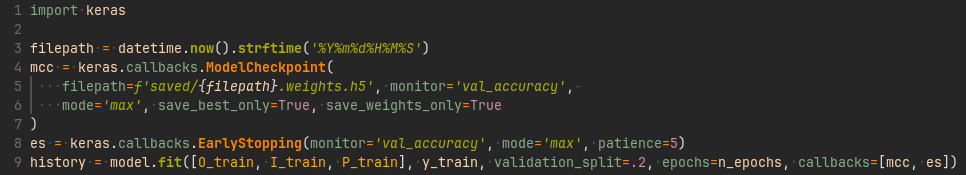
\includegraphics[width=\textwidth]{visuals/train.png}
      \caption{Snippet cu antrenarea modelului}
      \label{fig:train}
\end{figure}

\chapter{Rezultate experimentale}
\section{Descrierea procesului de testare}
\section{Rezultate experimentale}

\chapter{Concluzii, contribuţii şi direcţii de continuare a dezvoltării}
\section{Concluzii}
\section{Contribuții}
\section{Direcții viitoare}

\addcontentsline{toc}{chapter}{Bibliografie}
\bibliographystyle{plainnat}
\bibliography{bibliography}

\end{document}
